\documentclass[12pt, a4paper]{article}
\usepackage{triada}
\usepackage{subfigure}
\usepackage{float}
%\usepackage{enumerate}

\graphicspath{{eps/}{png/}}
\begin{document}

\section*{Задание 11}
\subsection*{Постановка}
Построить двумерное пуассоновское поле, отвечающее сложному пуассоновскому процессу:
\begin{enumerate}
	\item Первая интерпретация: система массового обслуживания. При этом, первая координата поля --- время поступления заявки в СМО (равномерное распределение), вторая --- время её обслуживания (распределение $\chi^2$ с $10$ степенями свободы).
	\item Вторая интерпретация: работа страховой компании. Первая координата --- момент наступления страхового случая (равномерное распределение), вторая --- величина ущерба (распределение Парето). Поступление капитала по времени линейно со скоростью $c>0$, начальный капитал $W>0$. Посчитать распределение времени разорения для различных значений параметров.
\end{enumerate}

\subsection*{Система массового обслуживания}
При равномерном распределении заявок разница между соседними (в смысле вариационного ряда) заявками можно считать экспоненциально распределённым с некоторым параметром интенсивности $\lambda$.

Алгоритм таков: с помощью экспоненциального распределения генерируются $t_i-t_{i-1}, i=1,\dots,N$ --- времена заявок, для каждой заявки генерируется $x_i$ --- время исполнения.
Затем происходит прямое моделирование процесса поступления и выполнения заявок.

Проанализируем значение параметра $\lambda$: математическое ожидание времени исполнения заявки равно $10$, а разницы между поступлениями заявок --- $\frac 1\lambda$. Поэтому если $\lambda<\frac 1{10}$, то очередь будет на большом промежутке времени стремиться к бесконечному количеству заявок, при $\lambda > \frac 1{10}$ размер очереди будет колебаться около нуля. При $\lambda = \frac 1 {10}$ будет некоторое переходное положение.

\subsection*{Работа страховой компании}
\begin{df}
	\textit{Распределение Парето} с параметрами $x_m$ и $k$ задается функцией распределения 
	\[F(x)=1-\left(\frac{x_m}{x} \right)^k\cdot[x\geqslant x_m].\]
\end{df}

Для построения датчика распределения Парето воспользуемся методом обратных функций: 
\[F^{-1}(y) = \frac{x_m}{(1-y)^{\frac{1}{k}}}.\]

Так как $y$ будет реализацией равномерной на $[0,1]$ случайной величины $Y$, то можно заменить $1-y \to y$, получится 
\[ X = \frac{x_m}{Y^\frac{1}{k}}.\]

Закон роста капитала выражается формулой
\[ u(t) = u_0 + ct - S(t),\]
где $c$ --- скорость роста, $u_0$ --- капитал в начальный момент, $S(t)$ --- размер выплат к моменту времени $t$, то есть, если моменты выплат обозначить за $t_i$, размеры выплат $x_i$, то \[S(t) = \sum\limits_{i:t_i\leqslant t}x_i.\]

Момент разорения --- это минимальное положительное $t$ такое, что $u(t)<0$.

Алгоритм для моделирования таков: генерируются времена поступлений исков, размеры исков, и моделируется процесс: в каждый момент нового иска добавляется линейный доход, затем вычитается сумма иска и проверяется разорение.

\subsection*{Практическая часть}

\begin{figure}[H]
\subfigure[$\lambda=0.05.$]{
\includegraphics[scale=0.45]{smo_l005_t500.eps}
}
\subfigure[$\lambda=0.2.$]{
\includegraphics[scale=0.45]{smo_l02_t500.eps}
}
\caption{Примеры работы СМО, $\lambda\ne 0.1$ на временном отрезке $[0,500]$. При $\lambda<0.1$ очередь не застаивается, при $\lambda>0.1$ очередь бесконечно увеличивается.}
\end{figure}

\begin{figure}[H]
\subfigure{
\includegraphics[scale=0.45]{smo_l01_t500_1.eps}
}
\subfigure{
\includegraphics[scale=0.45]{smo_l01_t500_2.eps}
}
\caption{Примеры работы СМО, $\lambda= 0.1$ на временном отрезке $[0,500]$. Заметно, что очередь может становиться достаточно большой, однако не уходит на бесконечность.}
\end{figure}

\begin{figure}[H]
\subfigure{
\includegraphics[scale=0.45]{ins_l02_k05_x015_u20_c2.eps}
}
\subfigure{
\includegraphics[scale=0.45]{inshist_l02_k05_x015_u20_c2_sz10000.eps}
}
\caption{Пример работы страховой компании и гистограмма времен разорения при выборке из $10^4$ процессов. $\lambda = 0.2, k=0.5, x_m=0.15, u_0 = 20, c=2.$}
\end{figure}

\begin{figure}[H]
\subfigure{
\includegraphics[scale=0.45]{ins_l05_k05_x015_u20_c2.eps}
}
\subfigure{
\includegraphics[scale=0.45]{inshist_l05_k05_x015_u20_c2_sz10000.eps}
}
\caption{Пример работы страховой компании и гистограмма времен разорения при выборке из $10^4$ процессов. $\lambda = 0.5, k=0.5, x_m=0.15, u_0 = 20, c=2.$}
\end{figure}

\begin{figure}[H]
\subfigure[$\lambda = 0.5, k=2, x_m=10, u_0 = 1000, c=1.$]{
\includegraphics[scale=0.45]{ins_l05_k2_x10_u1000_c1.eps}
}
\subfigure[$\lambda = 0.2, k=1, x_m=0.15, u_0 = 20, c=1.$]{
\includegraphics[scale=0.45]{ins_l02_k1_x015_u20_c1.eps}
}
\caption{Примеры работы страховой компании.}
\end{figure}

\bibliographystyle{sastyle}
\bibliography{library}
\end{document}
